\section{GA Outputs}
Some of the done tests are presented in this section. Presented outputs must be considered as examples of common algorithm behavior. For several runs with the same settings was got little different results. If it is not otherwise stated, all tests run under conditions defined in the section "Settings" with previously specified "Model Room". The axis symmetry was preferred because there was nicer look of the outputs. Only the fitness function (\ref{eq:fitV2EUB}) was used. There was not preferred any target value in most of the tests therefore the preferences factor $\alpha$ was set to $0.5$.

\subsection{Settings}

All GA settings are summarized in the Table~\ref{tab:GAsettings}. All tests ended after reaching 25\textsuperscript{th} generation. The best solution from each generation was saved in two specimens. The first one was not able to mutate and it only took the best chromosome from previous to the next generation. This method is called "Elitism". The second one was able to mutate with defined probabilities and its purpose was to try a little change in the best chromosome.

Other parent solutions for the recombination and mutation were taken by tournament selection. One tournament made random group of four solutions and took the one with the best fitness (minimum). This method avoided a premature convergence of the best solution. It was desirable to let the diversity among solutions at least in early populations. The crossovers were made only in one point and its probability was set to~$90 \%$.

\begin{table}[htb]
	\renewcommand{\arraystretch}{1.3}
	\caption{Genetic Algorithm Settings}
 	\label{tab:GAsettings}
	\centering
  \begin{tabular}{| l | c |}
    \hline
    \textbf{First Population} & Random logic vectors \\
    \hline
    \textbf{Termination Cond.} & Defined count of generations \\
    \hline
		\textbf{Count of Gen.} & $25$ \\
    \hline
		\textbf{Population Size} & $100$ \\
	\hline
		\textbf{Parent Selec.} & Tournament 1 of 4 \\
    \hline
		\textbf{Survival Selec.} & Elitism \\
	\hline
		\textbf{Recombination Type} & One point \\
    \hline
		\textbf{Recombination Prop.} & $90 \%$ \\
	\hline
		\textbf{Mutation Method} & Bit inversion \& Permutation\\
	\hline
		\textbf{Mutation Prop.} & $1 \%$ \\
	\hline
		& $10 \% \left( per \geq 1\right)$\\
		\textbf{Permutation Prop.} &  $0.349 \% \left( per \geq 2\right)$ \\
		&$0.004 \% \left( per = 3\right)$\\
    \hline
  \end{tabular}
\end{table}

\subsection{Symmetry Comparison}

The results for both types of symmetry are presented in Figures~\ref{fig:V010_S0}, \ref{fig:V010_S1} and Table~\ref{tab:symmetry}. The axis symmetry has nicer design from point of human view. The axis symmetry is more common for luminaire placement so it was further preferred. There is also less difference among several GA outputs with the same settings.

Both symmetries has the same count of luminaires and very close resulting values. It can be said, that the resulting values are almost independent on the type of symmetry. However the center symmetry has more points of freedom so its design in some cases (other room dimensions, other luminous intensity distribution curve etc.) consisted for 2 luminaries less than the axis symmetry. In cases where the optimal count of luminaires could be the same, then there was negligible results dependency on the type of symmetry.

The center symmetry placement reminds X shape. That was also very common during the tests. The target ratio R was set to 1 in presented tests. However the resulting ratio is about 0.8 in both cases of the symmetry. It means that the increasing of uniformity was cheaper than the increasing of the average illuminance. This phenomenon is dependent on the shape of luminous intensity distribution curve. For other curves would be the resulting ratio different.

\begin{table}[tb]
	\renewcommand{\arraystretch}{1.8}
	\caption{Results for symmetry comparison}
 	\label{tab:symmetry}
	\centering
  \begin{tabular}{| c | c | c |}
    \hline
    & \textbf{Center symmetry} & \textbf{Axis symmetry} \\
    \hline
    $\overline{E}_{m}$ (lx) & 501 & 506 \\
    \hline
		$U_0$ ($-$)& 0.74 & 0.74 \\
    \hline
		$C$ (-) & 16 & 16 \\
	\hline
		$R$ (-) & 0.80 & 0.82 \\
  \hline
  \end{tabular}
\end{table}

\begin{figure}[tb]
  \centering
  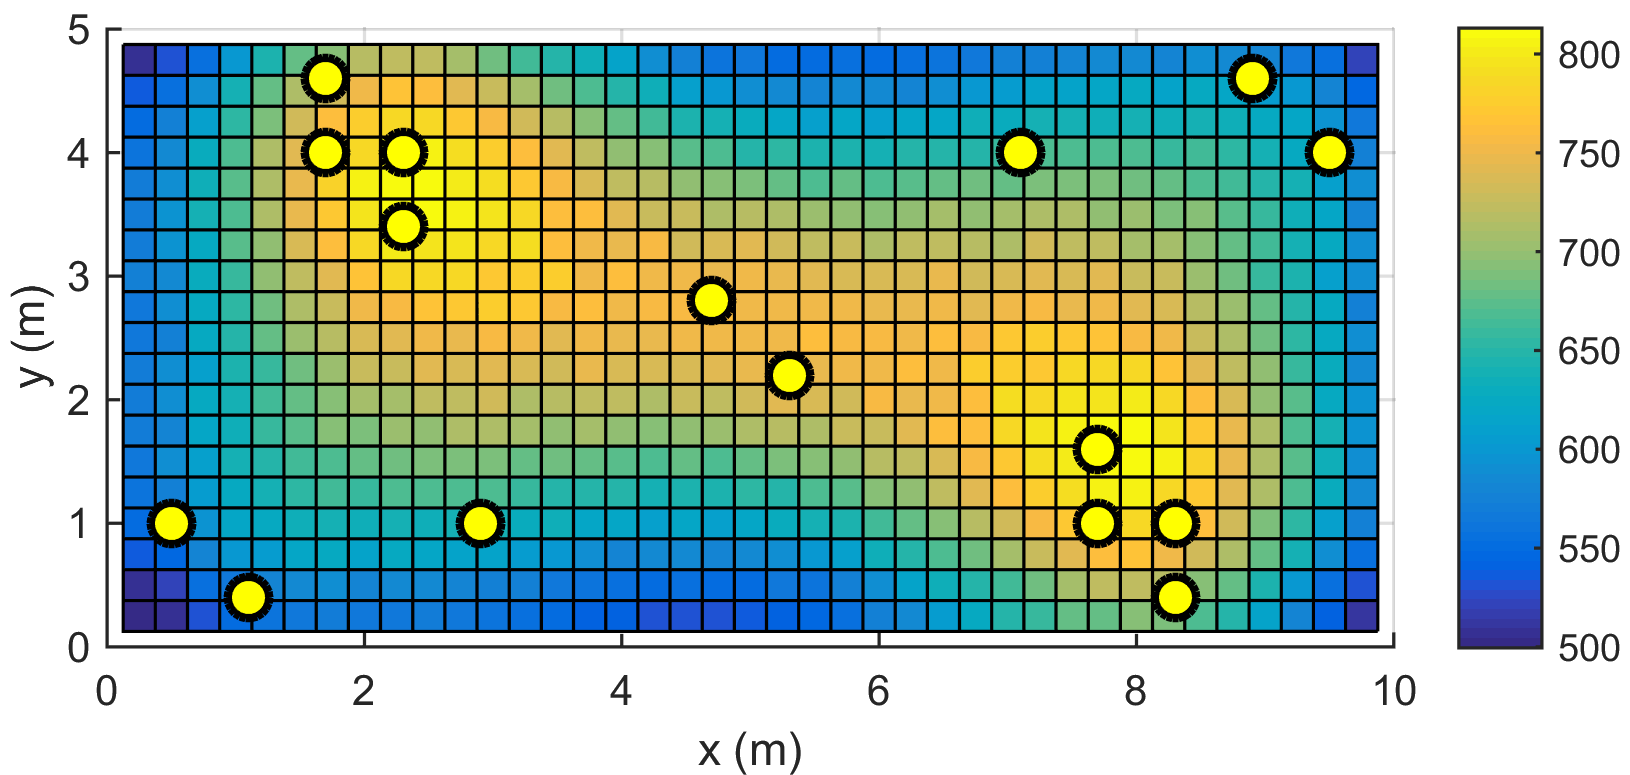
\includegraphics[width=\columnwidth]{MSTR_SLB_4x18W_5G4_Fit2_V010_S0}
  \caption{Luminaires placement with central symmetry}
  \label{fig:V010_S0}
\end{figure}

\begin{figure}[tb]
  \centering
  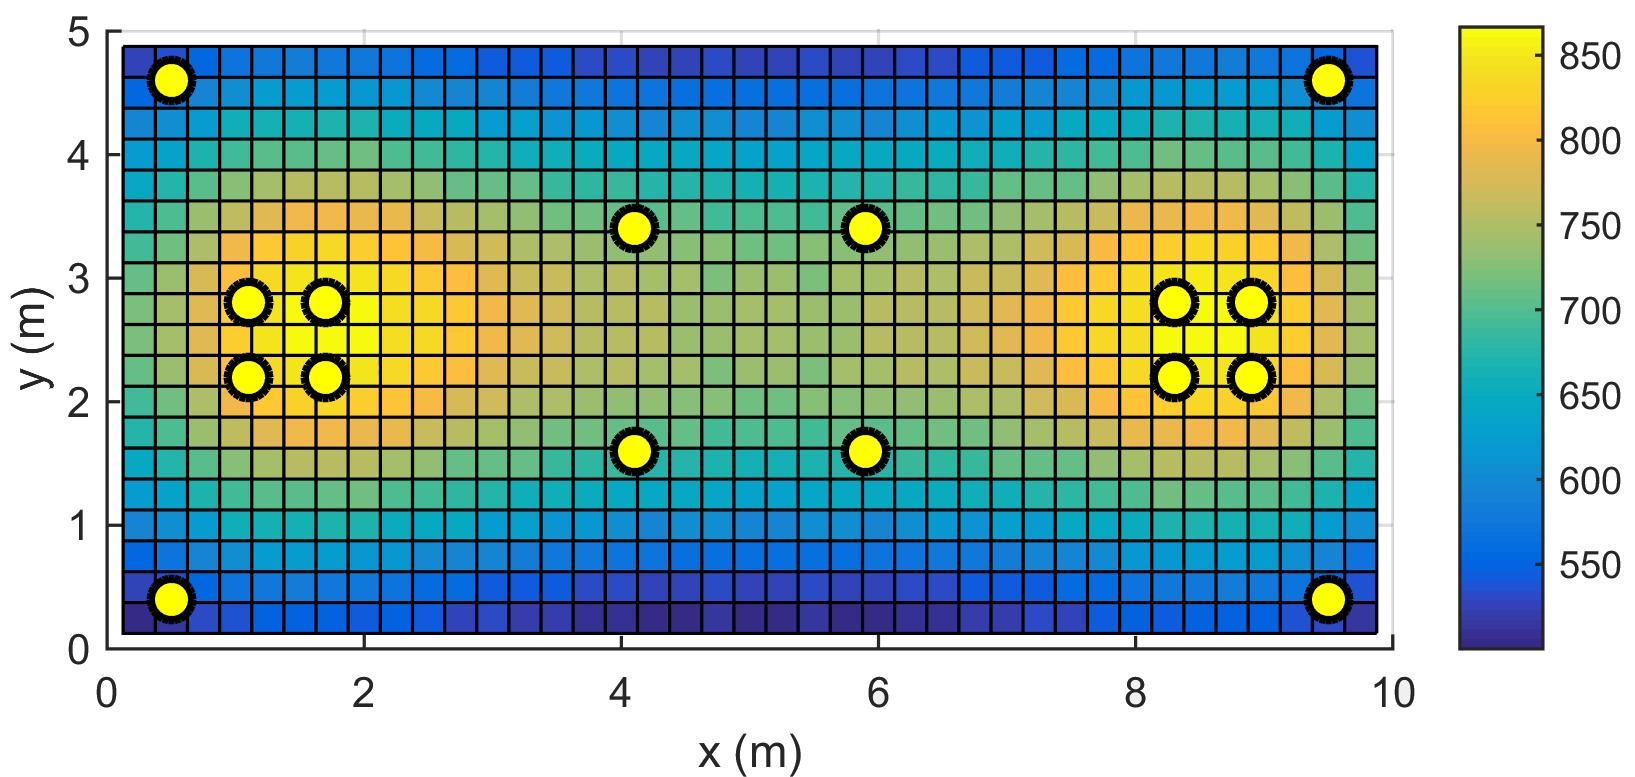
\includegraphics[width=\columnwidth]{../Vysledky/MSTR_SLB_4x18W_5G4_Fit2_V010_S1}
  \caption{Luminaires placement with axis symmetry}
  \label{fig:V010_S1}
\end{figure}

\subsection{Different Preferences}

The results for prefered value of average maintained illuminance and luminous uniformity are in Figures~\ref{fig:V010_S1_E}, \ref{fig:V010_S1_U} and Table~\ref{tab:preferences}. The results of not preferred parameter hit the minimal value given by the standard in both cases. The placement design for $\alpha = 0$ is more compressed around the center of the room (Figure~\ref{fig:V010_S1_E}). There is narrow area with high illuminace that increases the resulting average value of illuminance. The results for $\alpha = 1$ are very similar to the results with no preferences in Figure~\ref{fig:V010_S1} and Table~\ref{tab:symmetry}. This was common for the presented type of luminous intensity distribution curve. However after comparing all three ratios R, it can be seen, that highest one is in case of preferred illuminance and the lowest one is in the case of preferred uniformity.

\begin{table}[tb]
	\renewcommand{\arraystretch}{1.8}
	\caption{Results for different preferences}
 	\label{tab:preferences}
	\centering
  \begin{tabular}{| c | c | c |}
    \hline
    & $\alpha = 0$ & $\alpha = 1$ \\
    \hline
    $\overline{E}_{m}$ (lx) & 555 & 504 \\
    \hline
		$U_0$ ($-$)& 0.6 & 0.76 \\
    \hline
		$C$ (-) & 16 & 16 \\
	\hline
		$R$ (-) & 1.11 & 0.80 \\
  \hline
  \end{tabular}
\end{table}

\begin{figure}[tb]
  \centering
  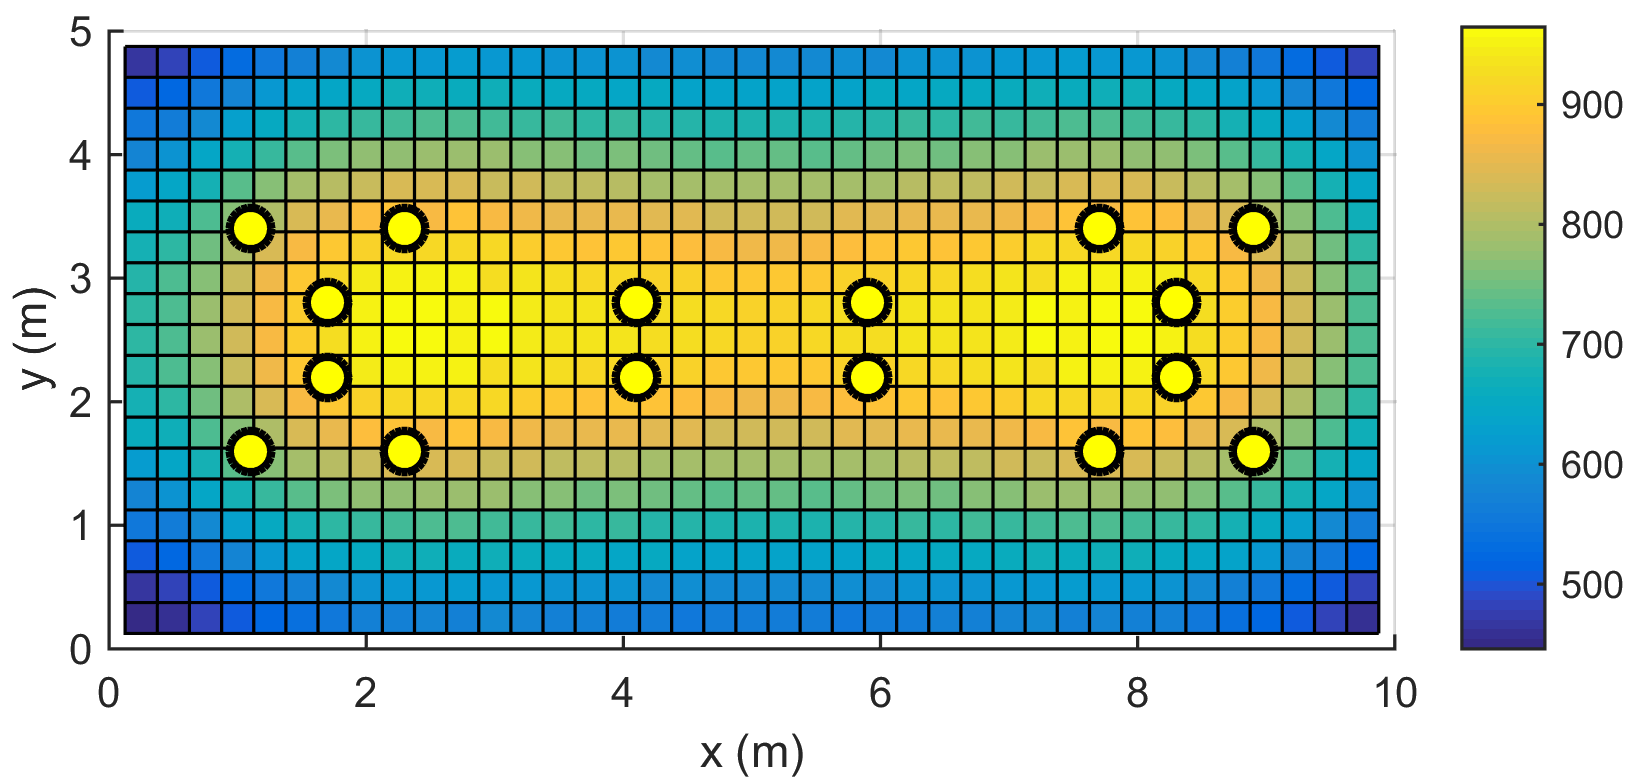
\includegraphics[width=\columnwidth]{../Vysledky/MSTR_SLB_4x18W_5G4_Fit2_E_V010_S1}
  \caption{Luminaires placement with prefered illuminance}
  \label{fig:V010_S1_E}
\end{figure}

\begin{figure}[tb]
  \centering
  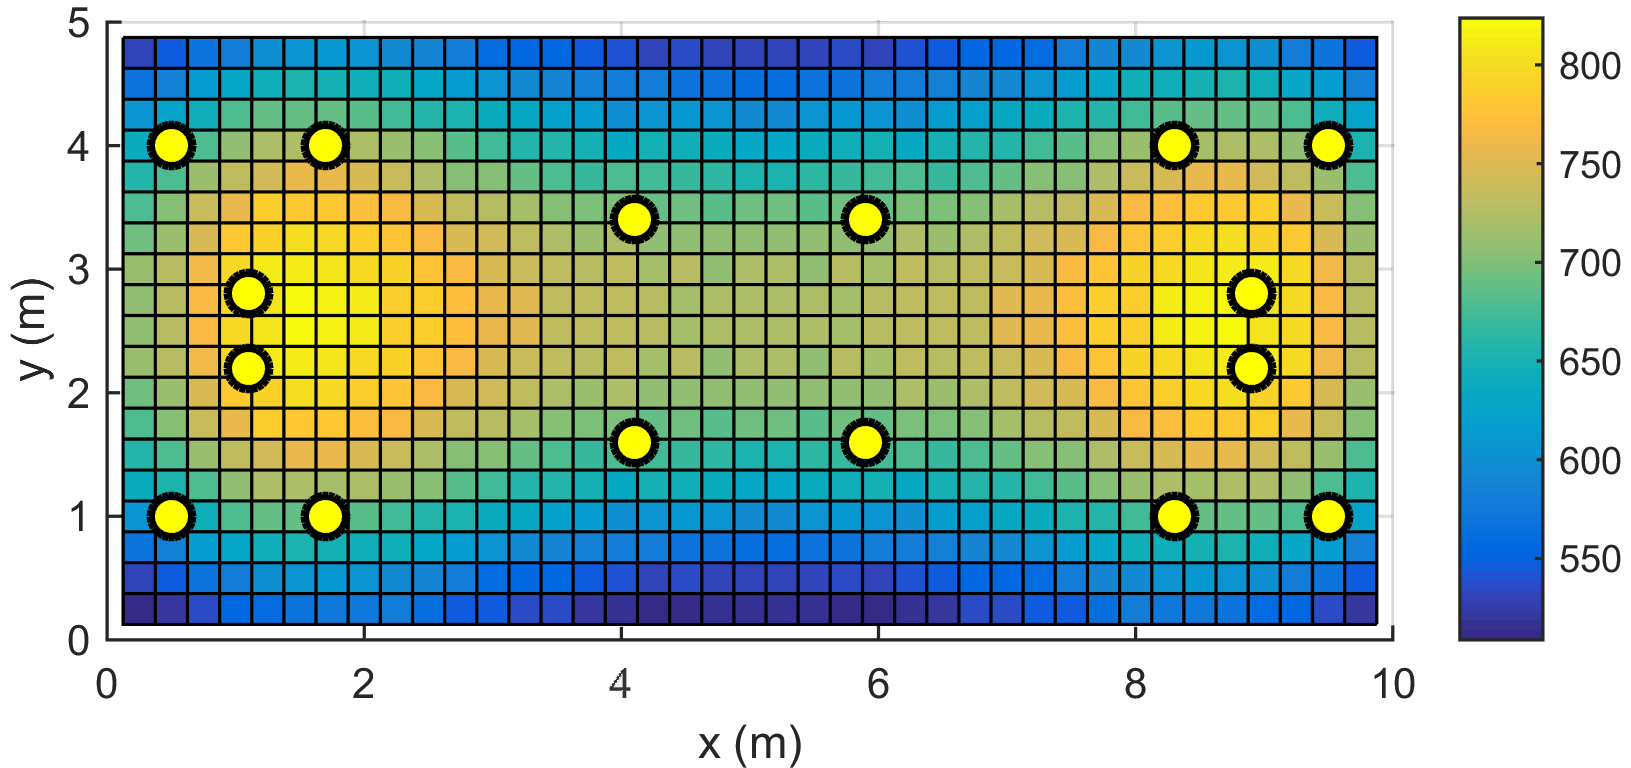
\includegraphics[width=\columnwidth]{../Vysledky/MSTR_SLB_4x18W_5G4_Fit2_U_V010_S1}
  \caption{Luminaires placement with prefered uniformity}
  \label{fig:V010_S1_U}
\end{figure}

\subsection{Without reflections}

The behavior of GA results if the reflections missing was tested too. The Design with no reflection is shown in Figure~\ref{fig:V010_S1_NoRef}. The case where the reflections missing only from the south wall is shown in Figure~\ref{fig:V010_S1_NoSWall}. The resulting watched values are presented in Table~\ref{tab:noRef}. The designed counts of luminaires C are higher in comparison to that from the equivalent case with all reflections from figure~\ref{fig:V010_S1} and Table~\ref{tab:symmetry}. Its common that the luminaires are placed closer to the walls now. For preferred uniformity were the distance from the walls even smaller. The asymmetric illuminace for symmetric luminaire placement can be seen in Figure~\ref{fig:V010_S1_NoSWall}. Both cases shows that the design is clearly affected be the presence of the reflections. Therefore there cannot be omitted from the algorithm.

\begin{table}[tb]
	\renewcommand{\arraystretch}{1.8}
	\caption{Results for missing reflections from any wall}
 	\label{tab:noRef}
	\centering
  \begin{tabular}{| c | c | c |}
    \hline
    & \textbf{Without walls} & \textbf{Without south wall} \\
    \hline
    $\overline{E}_{m}$ (lx) & 509 & 521 \\
    \hline
		$U_0$ ($-$)& 0.67 & 0.75 \\
    \hline
		$C$ (-) & 20 & 20 \\
	\hline
		$R$ (-) & 0.91 & 0.83 \\
  \hline
  \end{tabular}
\end{table}

\begin{figure}[tb]
  \centering
  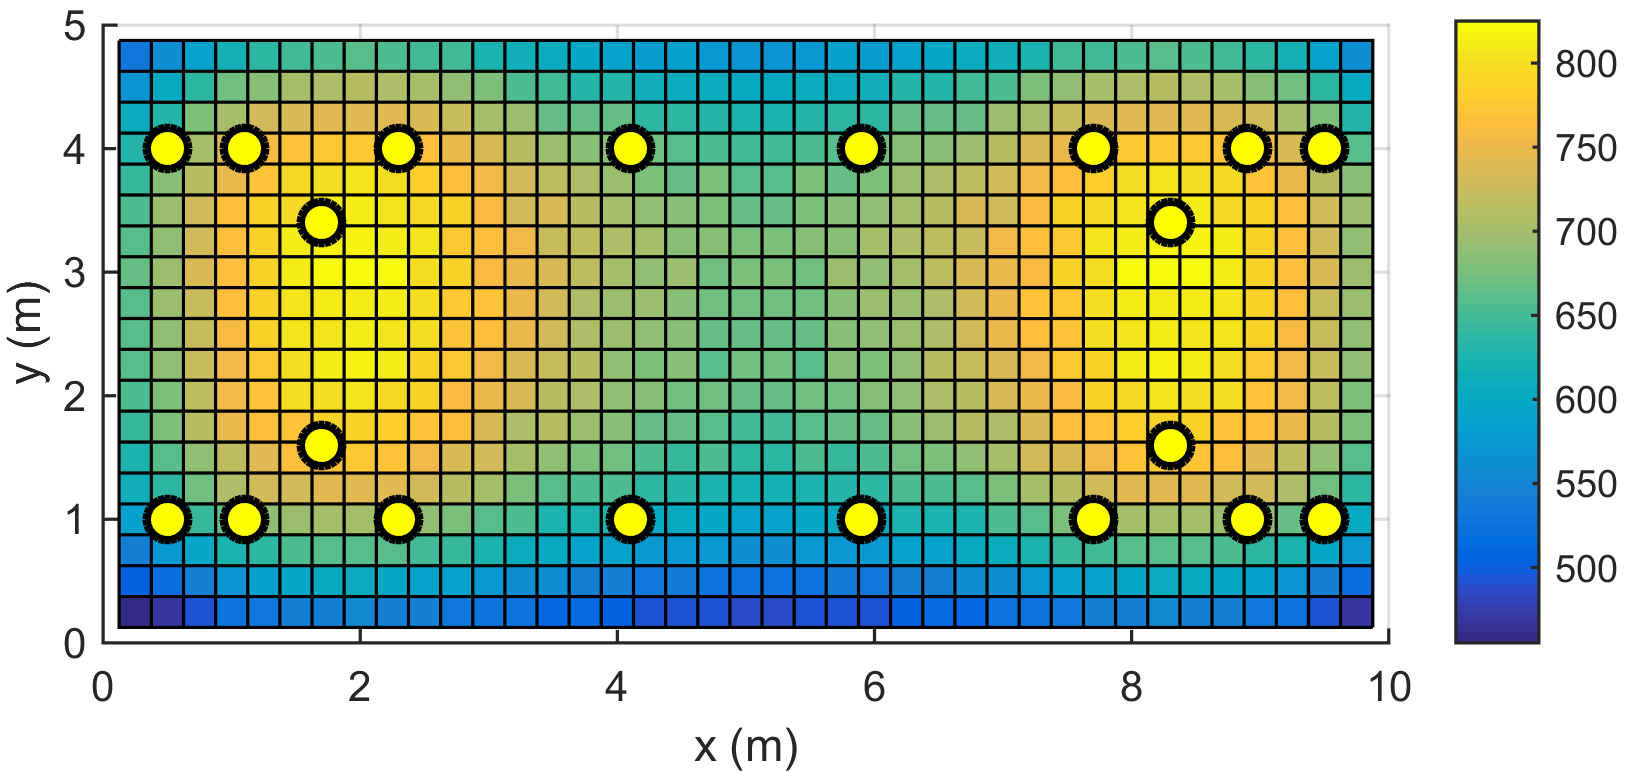
\includegraphics[width=\columnwidth]{../Vysledky/MSTR_SLB_4x18W_5G4_Fit2_NoRef_V010_S1}
  \caption{Luminaires placement without reflections from the walls and ceiling}
  \label{fig:V010_S1_NoRef}
\end{figure}

\begin{figure}[tb]
  \centering
  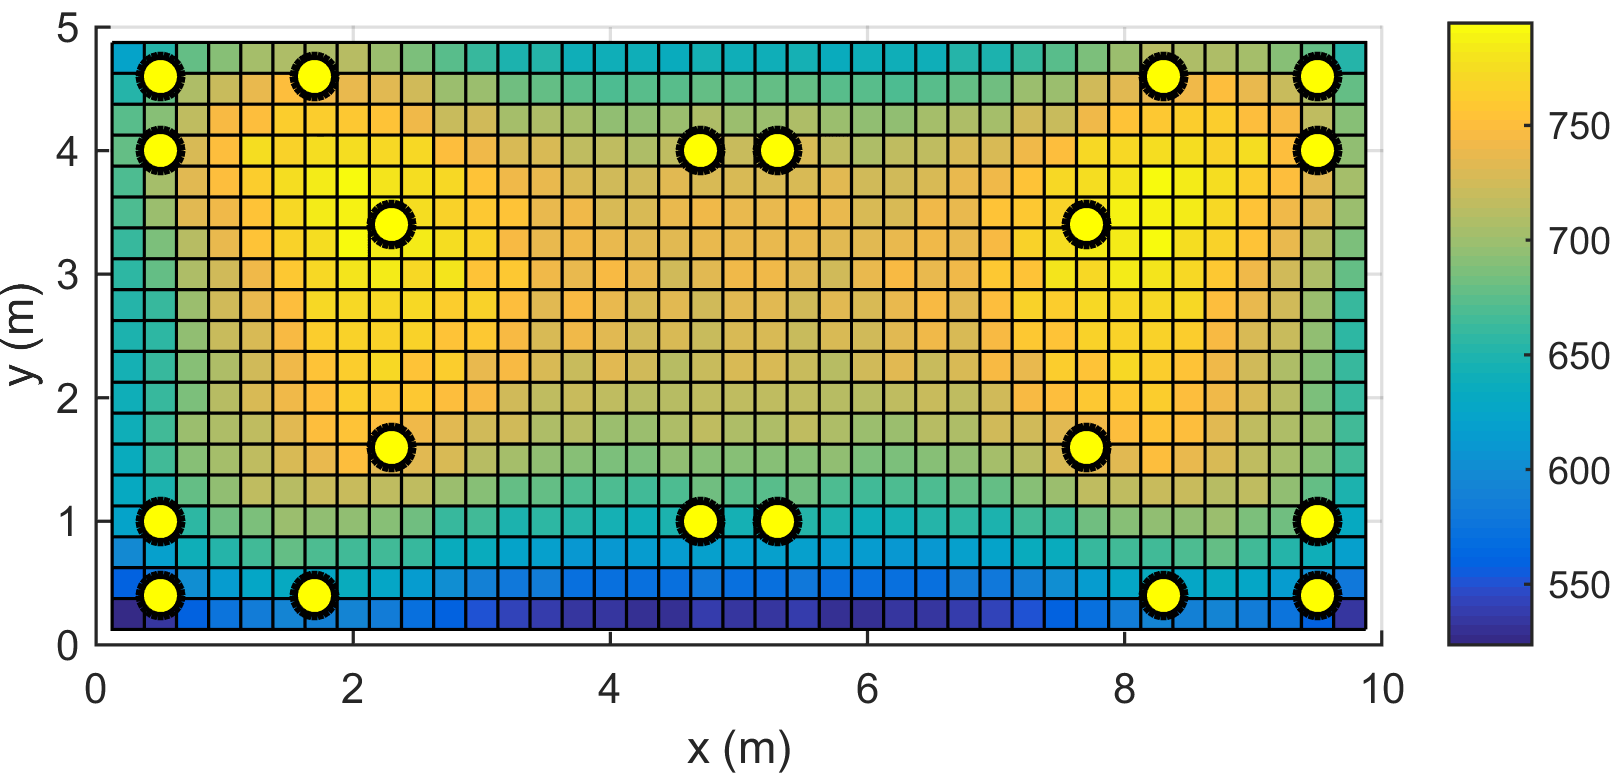
\includegraphics[width=\columnwidth]{../Vysledky/MSTR_SLB_4x18W_5G4_Fit2_NoSWall_V010_S1}
  \caption{Luminaires placement with no reflections from the south wall}
  \label{fig:V010_S1_NoSWall}
\end{figure}